\documentclass[12pt,a4paper]{article}
\usepackage[utf8]{inputenc}
\usepackage[portuguese]{babel}
\usepackage{indentfirst}
\usepackage{graphicx}
\usepackage{titling}
\usepackage{fancyhdr}
\usepackage{enumitem}
\usepackage{geometry}
\usepackage{xcolor}
\usepackage{tcolorbox}
\usepackage{float}
\usepackage{pdflscape}
\usepackage{hyperref}

% Configuração dos links no documento
\hypersetup{
    colorlinks=true,
    linkcolor=ufpeblue,
    filecolor=magenta,
    urlcolor=cyan,
    pdftitle={Sistema de Gerenciamento de Biblioteca Universitária},
    pdfpagemode=FullScreen,
}

% Configuração da página
\geometry{
    a4paper,
    top=2.5cm,
    bottom=2.5cm,
    left=3cm,
    right=3cm,
    headheight=14pt
}

% Configuração do cabeçalho
\pagestyle{fancy}
\fancyhf{}
\rhead{\thepage}
\lhead{Sistema de Biblioteca Universitária}
\renewcommand{\headrulewidth}{0.4pt}

% Definição das cores institucionais da UFPE
\definecolor{ufpeblue}{RGB}{0,47,108}

% Configuração de espaçamento para listas
\setlist{itemsep=0.5ex,parsep=0.5ex}

% Configuração das caixas coloridas
\tcbset{
    colback=gray!5,
    colframe=ufpeblue,
    arc=0mm,
    boxrule=0.5pt,
    fonttitle=\bfseries
}

% Título personalizado
\title{
    \vspace{-1.5cm}
    \begin{center}
        \large{UNIVERSIDADE FEDERAL DE PERNAMBUCO}\\
        \large{CENTRO DE INFORMÁTICA}\\
        \large{GRADUAÇÃO EM SISTEMAS DE INFORMAÇÃO}\\[2cm]
        \huge{\textbf{Sistema de Gerenciamento de Biblioteca Universitária}}\\[0.5cm]
        \large{Projeto da Disciplina IF976 - Banco de Dados}\\[4cm]
    \end{center}
}

\author{
    \begin{tabular}{c}
        Felipe Santos\\
        Juliana Serafim\\
        Matheus Dalia\\
        Pedro Balbino
    \end{tabular}
}

\date{Recife, Dezembro de 2024}

\begin{document}

\maketitle
\thispagestyle{empty}

\newpage
\tableofcontents
\thispagestyle{empty}
\newpage

\section{Introdução}
Este documento apresenta o projeto de banco de dados para um Sistema de Gerenciamento de Biblioteca Universitária, desenvolvido como parte da disciplina IF976 - Banco de Dados. O projeto está estruturado em quatro entregas principais:

\begin{enumerate}
    \item \textbf{Definição e descrição do minimundo} (09/12/2024)
    \item \textbf{Esquema conceitual} (11/12/2024)
    \item \textbf{Esquema relacional} (16/12/2024)
    \item \textbf{Lista de operações e consultas} (18/12/2024)
\end{enumerate}

Este documento contempla as duas primeiras entregas do projeto, apresentando tanto a descrição detalhada do minimundo quanto o esquema conceitual do banco de dados.



\section{Contextualização}
Este documento apresenta a primeira etapa do projeto da disciplina IF976 - Banco de Dados, que consiste no desenvolvimento de um sistema de gerenciamento para biblioteca universitária. O sistema proposto visa atender às necessidades específicas do ambiente acadêmico, facilitando o controle e a gestão do acervo bibliográfico.



\section{Descrição do Minimundo}

\subsection{Visão Geral}
\begin{tcolorbox}[title=Objetivo do Sistema]
O sistema tem como finalidade gerenciar de forma eficiente todos os aspectos operacionais de uma biblioteca universitária, desde o cadastro e controle do acervo até o gerenciamento de empréstimos e usuários.
\end{tcolorbox}

\subsection{Contexto}
A biblioteca universitária necessita de um sistema informatizado para automatizar seus processos internos e melhorar a qualidade dos serviços oferecidos à comunidade acadêmica. O sistema deve contemplar:

\begin{itemize}
    \item Gerenciamento completo do acervo bibliográfico
    \item Controle eficiente de empréstimos e devoluções
    \item Gestão de usuários (alunos, professores e funcionários)
    \item Sistema de multas e penalidades
    \item Geração de relatórios gerenciais e estatísticos
    \item Controle de acesso e segurança
\end{itemize}



\section{Estruturas Principais}

\subsection{Entidades e Seus Atributos}

\begin{tcolorbox}[title=Livro]
\begin{itemize}[leftmargin=*]
    \item \textbf{Identificação}:
    \begin{itemize}
        \item ISBN (chave primária)
        \item Código de tombamento
        \item Código de barras
    \end{itemize}
    \item \textbf{Informações Básicas}:
    \begin{itemize}
        \item Título
        \item Subtítulo
        \item Autor(es)
        \item Editora
        \item Edição
        \item Ano de publicação
    \end{itemize}
    \item \textbf{Categorização}:
    \begin{itemize}
        \item Área de conhecimento
        \item Palavras-chave
        \item Classificação (ex: livro, periódico, tese)
    \end{itemize}
    \item \textbf{Localização}:
    \begin{itemize}
        \item Seção
        \item Prateleira
        \item Posição
    \end{itemize}
    \item \textbf{Controle}:
    \begin{itemize}
        \item Quantidade de exemplares
        \item Status de conservação
        \item Data de aquisição
    \end{itemize}
\end{itemize}
\end{tcolorbox}

\begin{tcolorbox}[title=Usuário]
\begin{itemize}[leftmargin=*]
    \item \textbf{Dados Pessoais}:
    \begin{itemize}
        \item ID (chave primária)
        \item Nome completo
        \item CPF
        \item RG
        \item Data de nascimento
        \item Endereço completo
        \item Telefone(s)
        \item Email
    \end{itemize}
    \item \textbf{Dados Acadêmicos}:
    \begin{itemize}
        \item Tipo de vínculo (aluno, professor, funcionário)
        \item Curso/Departamento
        \item Número de matrícula/SIAPE
        \item Data de início do vínculo
    \end{itemize}
    \item \textbf{Dados do Sistema}:
    \begin{itemize}
        \item Login
        \item Senha
        \item Status da conta
        \item Histórico de empréstimos
        \item Situação de multas
    \end{itemize}
\end{itemize}
\end{tcolorbox}

\begin{tcolorbox}[title=Empréstimo]
\begin{itemize}[leftmargin=*]
    \item \textbf{Identificação}:
    \begin{itemize}
        \item Número do empréstimo (chave primária)
        \item ID do usuário (chave estrangeira)
        \item ISBN do livro (chave estrangeira)
    \end{itemize}
    \item \textbf{Datas}:
    \begin{itemize}
        \item Data do empréstimo
        \item Data prevista para devolução
        \item Data efetiva de devolução
    \end{itemize}
    \item \textbf{Controle}:
    \begin{itemize}
        \item Status do empréstimo
        \item Número de renovações
        \item Funcionário responsável
        \item Observações
    \end{itemize}
\end{itemize}
\end{tcolorbox}



\section{Regras de Negócio}

\begin{enumerate}[label=\textbf{RN\arabic*.}, leftmargin=*]
    \item \textbf{Empréstimos}
    \begin{itemize}
        \item Professores podem emprestar até 7 livros por 30 dias
        \item Alunos podem emprestar até 5 livros por 15 dias
        \item Funcionários podem emprestar até 3 livros por 15 dias
        \item Renovações são permitidas até 2 vezes, se não houver reserva
        \item Um exemplar só pode ser emprestado se não estiver reservado
    \end{itemize}

    \item \textbf{Multas e Penalidades}
    \begin{itemize}
        \item Multa diária por atraso de R\$ 1,00 por livro
        \item Bloqueio de novos empréstimos para usuários com multas pendentes
        \item Após 30 dias de atraso, suspensão do direito de empréstimo por 60 dias
        \item Sistema deve enviar notificações automáticas de atraso
    \end{itemize}

    \item \textbf{Reservas}
    \begin{itemize}
        \item Limite de 3 reservas simultâneas por usuário
        \item Reserva válida por 24 horas após a devolução do livro
        \item Ordem de prioridade por data de solicitação
    \end{itemize}

    \item \textbf{Cadastro e Manutenção}
    \begin{itemize}
        \item Todos os livros devem ter ISBN válido
        \item Usuários devem manter dados cadastrais atualizados
        \item Baixa de livros só pode ser feita por bibliotecários
        \item Inventário anual obrigatório
    \end{itemize}
\end{enumerate}



\section{Operações do Sistema}

\begin{tcolorbox}[title=Operações Principais]
\begin{enumerate}[label=\textbf{OP\arabic*.}]
    \item \textbf{Gestão de Acervo}
    \begin{itemize}
        \item Cadastro de novos livros
        \item Atualização de informações bibliográficas
        \item Controle de exemplares
        \item Baixa de material
        \item Inventário
    \end{itemize}

    \item \textbf{Controle de Empréstimos}
    \begin{itemize}
        \item Registro de empréstimos
        \item Renovações
        \item Devoluções
        \item Reservas
        \item Controle de atrasos
    \end{itemize}

    \item \textbf{Gestão de Usuários}
    \begin{itemize}
        \item Cadastro de novos usuários
        \item Atualização de dados cadastrais
        \item Controle de situação (ativo/inativo)
        \item Histórico de empréstimos
        \item Gestão de multas
    \end{itemize}

    \item \textbf{Relatórios e Estatísticas}
    \begin{itemize}
        \item Relatórios de movimentação
        \item Estatísticas de uso
        \item Relatórios de multas
        \item Histórico de operações
        \item Indicadores de desempenho
    \end{itemize}

    \item \textbf{Administração do Sistema}
    \begin{itemize}
        \item Controle de acesso
        \item Backup de dados
        \item Configurações do sistema
        \item Logs de operações
        \item Manutenção do sistema
    \end{itemize}
\end{enumerate}
\end{tcolorbox}



\section{Esquema Conceitual}

\subsection{Desenvolvimento do Modelo ER}
O esquema conceitual foi desenvolvido seguindo as etapas de modelagem Entidade-Relacionamento, identificando os principais componentes do sistema e suas interações. O processo incluiu:

\begin{enumerate}
    \item Identificação das entidades regulares e fracas
    \item Definição dos atributos (simples, compostos e multivalorados)
    \item Estabelecimento dos relacionamentos
    \item Determinação das cardinalidades
    \item Análise das especializações/generalizações necessárias
\end{enumerate}

\subsection{Entidades}
\begin{tcolorbox}[title=Identificação das Entidades]
\begin{itemize}
    \item \textbf{Entidades Fortes}:
    \begin{itemize}
        \item LIVRO: representa a obra bibliográfica
        \item USUÁRIO: representa os usuários do sistema
        \item FUNCIONÁRIO: representa os funcionários da biblioteca
    \end{itemize}
    \item \textbf{Entidades Fracas}:
    \begin{itemize}
        \item EXEMPLAR: depende da existência de um LIVRO
        \item EMPRÉSTIMO: depende de USUÁRIO e EXEMPLAR
    \end{itemize}
\end{itemize}
\end{tcolorbox}

\subsection{Atributos}
\begin{tcolorbox}[title=Tipos de Atributos]

\subsubsection{Atributos Identificadores}
\begin{itemize}
    \item LIVRO: ISBN (chave primária)
    \item USUÁRIO: ID, CPF (chaves candidatas)
    \item EXEMPLAR: Código de Tombamento + ISBN (chave parcial + chave do proprietário)
    \item EMPRÉSTIMO: ID do empréstimo (chave artificial)
\end{itemize}

\subsubsection{Atributos Compostos}
\begin{itemize}
    \item Endereço (logradouro, número, complemento, bairro, cidade, estado, CEP)
    \item Nome Completo (primeiro nome, sobrenome)
\end{itemize}

\subsubsection{Atributos Multivalorados}
\begin{itemize}
    \item Telefone(s)
    \item Autor(es)
    \item Palavras-chave
\end{itemize}

\subsubsection{Atributos Derivados}
\begin{itemize}
    \item Idade (derivado da data de nascimento)
    \item Tempo de empréstimo (derivado das datas de empréstimo e devolução)
    \item Valor da multa (derivado do tempo de atraso)
\end{itemize}
\end{tcolorbox}

\subsection{Relacionamentos}
\begin{tcolorbox}[title=Tipos de Relacionamentos]
\subsubsection{Relacionamentos Binários}
\begin{itemize}
    \item \textbf{POSSUI} (LIVRO-EXEMPLAR)
    \begin{itemize}
        \item Tipo: 1:N
        \item Participação total do lado EXEMPLAR
        \item Atributos: nenhum
    \end{itemize}

    \item \textbf{REALIZA} (USUÁRIO-EMPRÉSTIMO)
    \begin{itemize}
        \item Tipo: 1:N
        \item Participação total do lado EMPRÉSTIMO
        \item Atributos: nenhum
    \end{itemize}

    \item \textbf{PARTICIPA} (EXEMPLAR-EMPRÉSTIMO)
    \begin{itemize}
        \item Tipo: 1:N
        \item Participação total do lado EMPRÉSTIMO
        \item Atributos: data\_empréstimo, data\_devolução\_prevista
    \end{itemize}

    \item \textbf{CADASTRA} (FUNCIONÁRIO-EMPRÉSTIMO)
    \begin{itemize}
        \item Tipo: 1:N
        \item Participação total do lado EMPRÉSTIMO
        \item Atributos: data\_cadastro
    \end{itemize}
\end{itemize}

\subsubsection{Restrições de Participação}
\begin{itemize}
    \item EXEMPLAR deve pertencer a um LIVRO (participação total)
    \item EMPRÉSTIMO deve ter um USUÁRIO e um EXEMPLAR (participação total)
    \item EMPRÉSTIMO deve ser cadastrado por um FUNCIONÁRIO (participação total)
\end{itemize}
\end{tcolorbox}

\subsection{Diagrama ER}
A seguir, apresentamos o diagrama ER completo do sistema, que representa todas as entidades, relacionamentos e atributos identificados para o Sistema de Gerenciamento de Biblioteca Universitária:

% Página em paisagem para o diagrama
\begin{landscape}
\begin{figure}[]
    \centering
    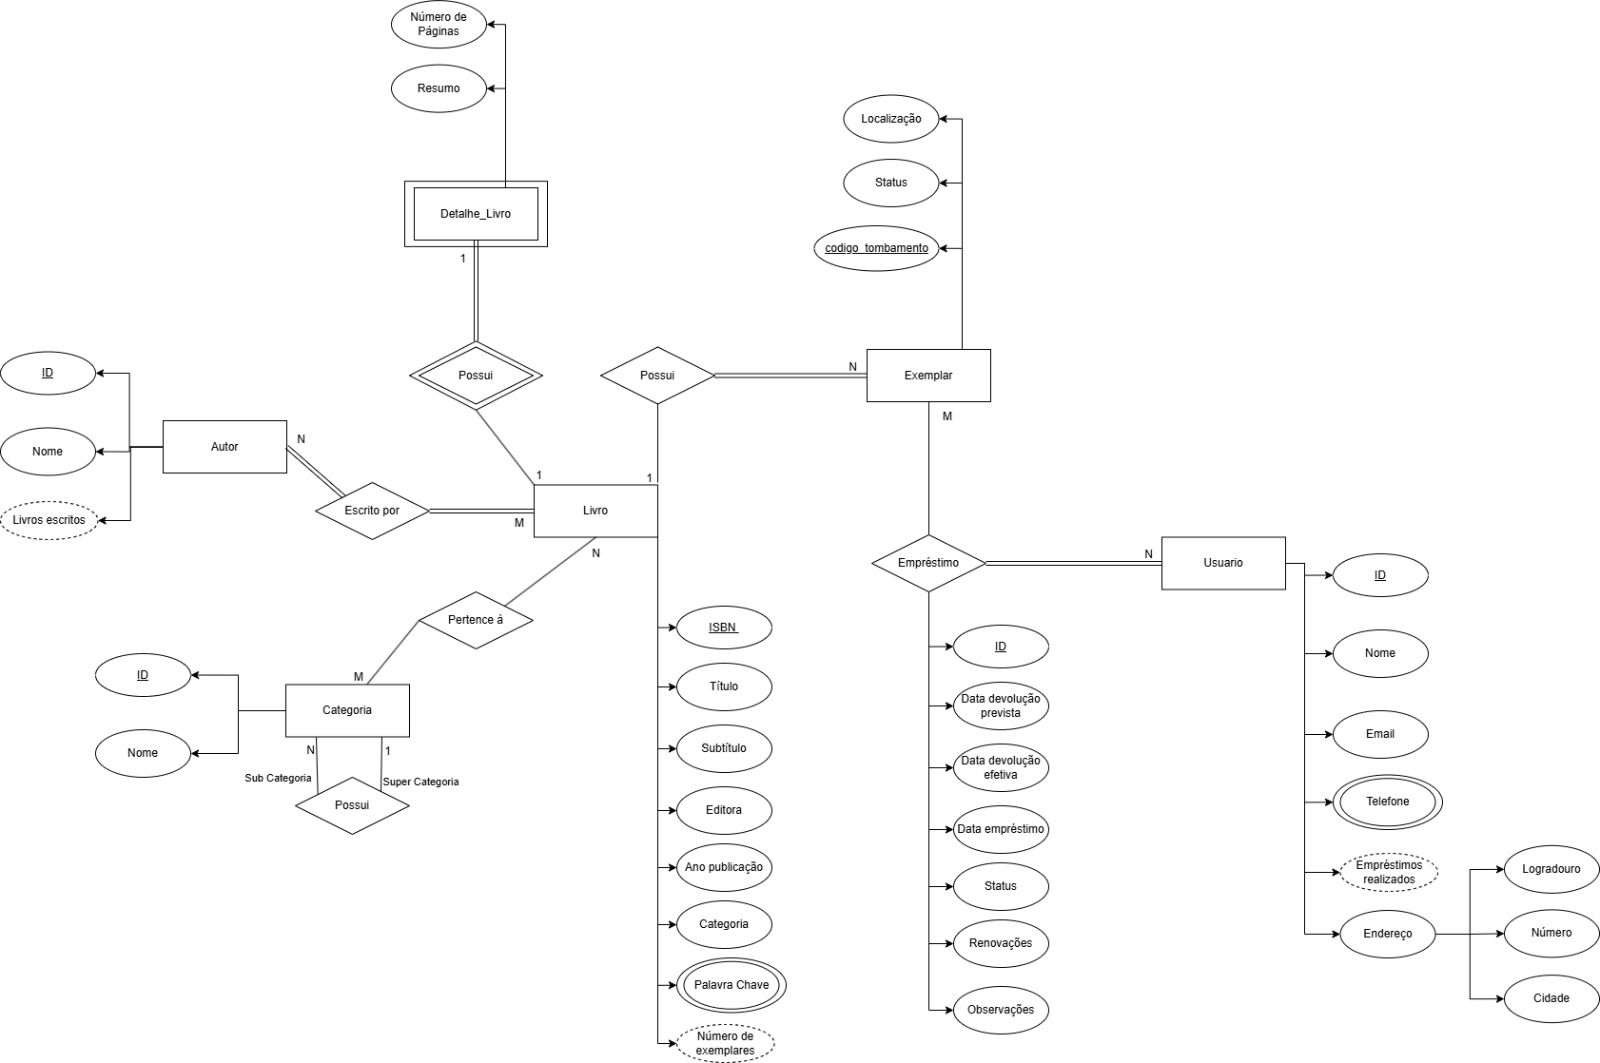
\includegraphics[width=0.95\linewidth]{ModeloConceitual.png}
    \caption{Diagrama Entidade-Relacionamento do Sistema de Biblioteca}
    \label{fig:diagrama-er}
\end{figure}
\end{landscape}

\subsubsection{Detalhamento dos Elementos}
\begin{tcolorbox}[title=Elementos do Diagrama]
\begin{enumerate}
    \item \textbf{Entidade Livro}
    \begin{itemize}
        \item Chave primária: ISBN
        \item Atributos descritivos: título, subtítulo, editora, edição
        \item Atributos de categorização: área de conhecimento, palavras-chave
    \end{itemize}

    \item \textbf{Entidade Exemplar}
    \begin{itemize}
        \item Identificação: código de tombamento, código de barras
        \item Controle: status de conservação, data de aquisição
        \item Localização: seção, prateleira, posição
    \end{itemize}

    \item \textbf{Entidade Usuário}
    \begin{itemize}
        \item Identificadores: ID, CPF, RG
        \item Dados pessoais: nome completo, data de nascimento, endereço
        \item Especialização em: Aluno, Professor e Funcionário
    \end{itemize}

    \item \textbf{Entidade Empréstimo}
    \begin{itemize}
        \item Controle temporal:
        \begin{itemize}
            \item Data do empréstimo
            \item Data prevista para devolução
            \item Data efetiva de devolução
        \end{itemize}
        \item Gestão:
        \begin{itemize}
            \item Status do empréstimo
            \item Número de renovações
            \item Observações
        \end{itemize}
        \item Rastreamento:
        \begin{itemize}
            \item Funcionário responsável
            \item ID do empréstimo
        \end{itemize}
    \end{itemize}
\end{enumerate}
\end{tcolorbox}

\subsection{Relacionamentos Principais}

\begin{tcolorbox}[title=Relacionamentos do Sistema]
\begin{enumerate}[label=\textbf{R\arabic*.}]
    \item \textbf{Livro-Exemplar (Possui)}
    \begin{itemize}
        \item Cardinalidade: 1:N
        \item Um livro pode ter vários exemplares
        \item Cada exemplar pertence a exatamente um livro
    \end{itemize}

    \item \textbf{Exemplar-Empréstimo (Participa)}
    \begin{itemize}
        \item Cardinalidade: 1:N
        \item Um exemplar pode participar de vários empréstimos (em momentos diferentes)
        \item Cada empréstimo está associado a exatamente um exemplar
    \end{itemize}

    \item \textbf{Usuário-Empréstimo (Realiza)}
    \begin{itemize}
        \item Cardinalidade: 1:N
        \item Um usuário pode realizar vários empréstimos
        \item Cada empréstimo está associado a exatamente um usuário
    \end{itemize}

    \item \textbf{Funcionário-Empréstimo (Cadastrado\_por)}
    \begin{itemize}
        \item Cardinalidade: 1:N
        \item Um funcionário pode cadastrar vários empréstimos
        \item Cada empréstimo é cadastrado por exatamente um funcionário
    \end{itemize}
\end{enumerate}
\end{tcolorbox}

\subsection{Especializações/Generalizações}
\begin{tcolorbox}[title=Hierarquia de Especialização]

\subsubsection{Especialização de USUÁRIO}
\begin{itemize}
    \item Tipo: Disjunta (d)
    \item Completude: Total
    \item Critério: Tipo de vínculo com a instituição
    \item Subclasses:
    \begin{itemize}
        \item ALUNO
        \begin{itemize}
            \item Atributos específicos: número\_matrícula, curso
        \end{itemize}
        \item PROFESSOR
        \begin{itemize}
            \item Atributos específicos: SIAPE, departamento
        \end{itemize}
        \item FUNCIONÁRIO
        \begin{itemize}
            \item Atributos específicos: SIAPE, setor
        \end{itemize}
    \end{itemize}
\end{itemize}

\subsubsection{Justificativa da Especialização}
A especialização foi escolhida porque:
\begin{itemize}
    \item Cada tipo de usuário tem atributos específicos
    \item As regras de empréstimo variam por tipo
    \item Um usuário não pode pertencer a múltiplas categorias
    \item Todo usuário deve ser classificado em uma categoria
\end{itemize}

\begin{itemize}
    \item \textbf{Aluno}
    \begin{itemize}
        \item Atributos específicos: número de matrícula, curso
        \item Limite de empréstimo: 5 livros
        \item Prazo de empréstimo: 15 dias
    \end{itemize}

    \item \textbf{Professor}
    \begin{itemize}
        \item Atributos específicos: SIAPE, departamento
        \item Limite de empréstimo: 7 livros
        \item Prazo de empréstimo: 30 dias
    \end{itemize}

    \item \textbf{Funcionário}
    \begin{itemize}
        \item Atributos específicos: SIAPE, departamento
        \item Limite de empréstimo: 3 livros
        \item Prazo de empréstimo: 15 dias
    \end{itemize}
\end{itemize}
\end{tcolorbox}




\section{Esquema Relacional}

\subsection{Processo de Mapeamento}
O esquema relacional foi desenvolvido a partir do modelo conceitual (ER) seguindo as regras de mapeamento estabelecidas na literatura. O processo incluiu:

\begin{enumerate}
    \item Mapeamento de entidades regulares
    \item Mapeamento de entidades fracas
    \item Mapeamento de relacionamentos
    \item Tratamento de especializações
    \item Mapeamento de atributos multivalorados
    \item Mapeamento de atributos compostos
\end{enumerate}

\subsection{Diagrama do Banco de Dados}
A Figura \ref{fig:modelo-relacional} apresenta o diagrama do esquema relacional completo, ilustrando todas as tabelas, seus relacionamentos e as chaves primárias e estrangeiras do sistema.

\begin{figure}[H]
    \centering
    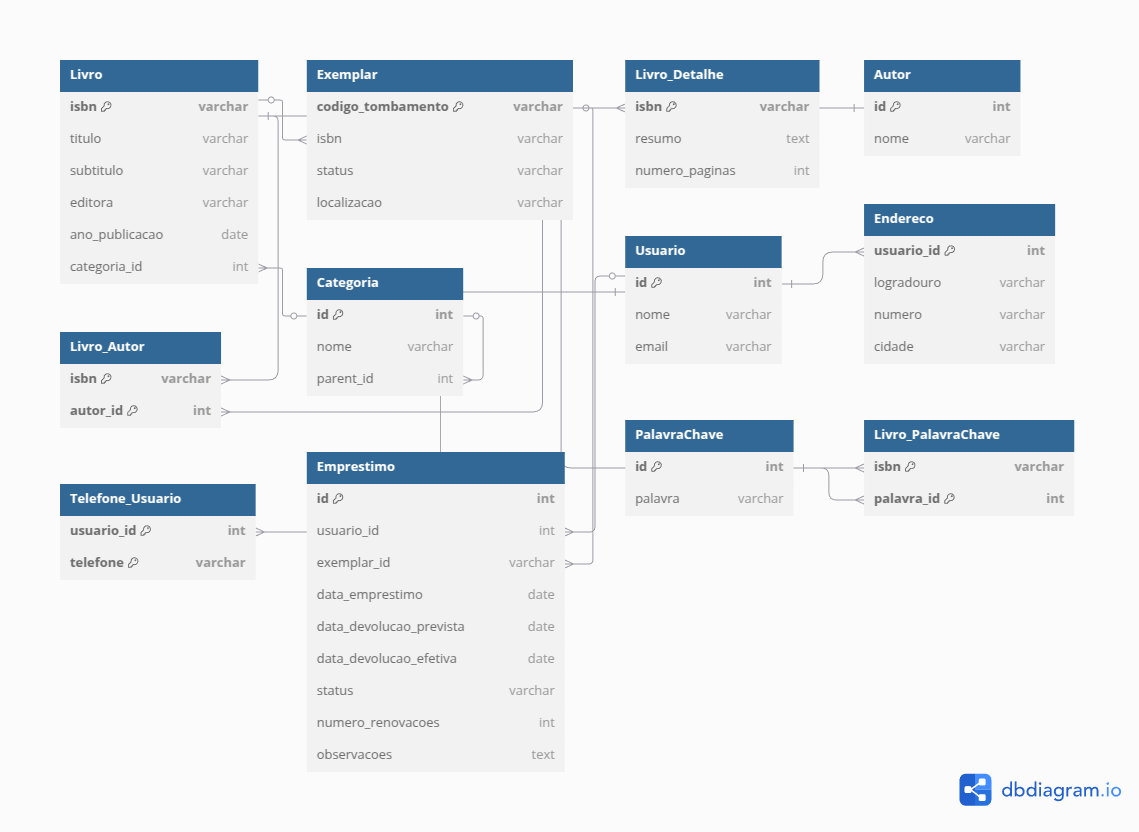
\includegraphics[width=\textwidth]{ModeloRelacional.png}
    \caption{Diagrama do Esquema Relacional do Sistema de Biblioteca}
    \label{fig:modelo-relacional}
\end{figure}

\subsection{Relações Resultantes}

\begin{tcolorbox}[title=Entidades Principais]
\begin{itemize}
    \item \textbf{LIVRO} (\underline{isbn}, titulo, subtitulo, editora, edicao, ano\_publicacao, area\_conhecimento, data\_cadastro)

    \item \textbf{EXEMPLAR} (\underline{codigo\_tombamento}, isbn[\textit{FK}], codigo\_barras, status\_conservacao, data\_aquisicao, secao, prateleira, posicao)

    \item \textbf{USUARIO} (\underline{id}, tipo\_usuario, nome, cpf, rg, data\_nascimento, email, login, senha, status\_conta)
\end{itemize}
\end{tcolorbox}

\begin{tcolorbox}[title=Especializações]
\begin{itemize}
    \item \textbf{ALUNO} (\underline{id}[\textit{FK}], numero\_matricula, curso)

    \item \textbf{PROFESSOR} (\underline{id}[\textit{FK}], siape, departamento)

    \item \textbf{FUNCIONARIO} (\underline{id}[\textit{FK}], siape, setor)
\end{itemize}
\end{tcolorbox}

\begin{tcolorbox}[title=Relacionamentos]
\begin{itemize}
    \item \textbf{EMPRESTIMO} (\underline{id}, usuario\_id[\textit{FK}], exemplar\_codigo[\textit{FK}], funcionario\_id[\textit{FK}], data\_emprestimo, data\_devolucao\_prevista, data\_devolucao\_efetiva, status, numero\_renovacoes, observacoes)

    \item \textbf{RESERVA} (\underline{id}, usuario\_id[\textit{FK}], exemplar\_codigo[\textit{FK}], data\_reserva, data\_validade, status)

    \item \textbf{MULTA} (\underline{id}, emprestimo\_id[\textit{FK}], valor, status, data\_geracao, data\_pagamento)
\end{itemize}
\end{tcolorbox}

\begin{tcolorbox}[title=Atributos Multivalorados]
\begin{itemize}
    \item \textbf{TELEFONE\_USUARIO} (\underline{usuario\_id[\textit{FK}]}, \underline{telefone})

    \item \textbf{AUTOR\_LIVRO} (\underline{isbn[\textit{FK}]}, \underline{autor})

    \item \textbf{PALAVRACHAVE\_LIVRO} (\underline{isbn[\textit{FK}]}, \underline{palavra\_chave})
\end{itemize}
\end{tcolorbox}

\begin{tcolorbox}[title=Atributos Compostos]
\begin{itemize}
    \item \textbf{ENDERECO\_USUARIO} (\underline{usuario\_id[\textit{FK}]}, logradouro, numero, complemento, bairro, cidade, estado, cep)
\end{itemize}
\end{tcolorbox}

\newpage
\subsection{Implementação em PostgreSQL}
O esquema do banco de dados foi implementado utilizando PostgreSQL, um sistema de gerenciamento de banco de dados relacional robusto e de código aberto. A seguir, apresentamos o código SQL completo para a criação do esquema, dividido em seções lógicas:

\begin{tcolorbox}[title=1. Entidades Principais,size=small]
\begin{verbatim}
-- Criação das tabelas principais
CREATE TABLE "Livro" (
    "isbn" VARCHAR(13) PRIMARY KEY,
    "titulo" VARCHAR(255) NOT NULL,
    "subtitulo" VARCHAR(255),
    "editora" VARCHAR(100) NOT NULL,
    "edicao" VARCHAR(50),
    "ano_publicacao" DATE NOT NULL,
    "area_conhecimento" VARCHAR(100) NOT NULL,
    "data_cadastro" DATE NOT NULL DEFAULT CURRENT_DATE
);

CREATE TABLE "Exemplar" (
    "codigo_tombamento" VARCHAR(20) PRIMARY KEY,
    "isbn" VARCHAR(13) NOT NULL,
    "codigo_barras" VARCHAR(50) UNIQUE,
    "status_conservacao" VARCHAR(20) NOT NULL,
    "data_aquisicao" DATE NOT NULL,
    "secao" VARCHAR(50) NOT NULL,
    "prateleira" VARCHAR(20) NOT NULL,
    "posicao" VARCHAR(20) NOT NULL,
    FOREIGN KEY ("isbn") REFERENCES "Livro" ("isbn")
);
\end{verbatim}
\end{tcolorbox}

\begin{tcolorbox}[title=2. Usuários e Especializações,size=small]
\begin{verbatim}
CREATE TABLE "Usuario" (
    "id" SERIAL PRIMARY KEY,
    "tipo_usuario" VARCHAR(20) NOT NULL,
    "nome" VARCHAR(100) NOT NULL,
    "cpf" VARCHAR(11) UNIQUE NOT NULL,
    "rg" VARCHAR(20) NOT NULL,
    "data_nascimento" DATE NOT NULL,
    "email" VARCHAR(100) UNIQUE NOT NULL,
    "login" VARCHAR(50) UNIQUE NOT NULL,
    "senha" VARCHAR(255) NOT NULL,
    "status_conta" VARCHAR(20) NOT NULL DEFAULT 'ATIVO',
    CONSTRAINT "chk_tipo_usuario"
        CHECK (tipo_usuario IN ('ALUNO', 'PROFESSOR', 'FUNCIONARIO'))
);

CREATE TABLE "Aluno" (
    "id" INTEGER PRIMARY KEY REFERENCES "Usuario" ("id") ON DELETE CASCADE,
    "numero_matricula" VARCHAR(20) UNIQUE NOT NULL,
    "curso" VARCHAR(100) NOT NULL
);

CREATE TABLE "Professor" (
    "id" INTEGER PRIMARY KEY REFERENCES "Usuario" ("id") ON DELETE CASCADE,
    "siape" VARCHAR(20) UNIQUE NOT NULL,
    "departamento" VARCHAR(100) NOT NULL
);

CREATE TABLE "Funcionario" (
    "id" INTEGER PRIMARY KEY REFERENCES "Usuario" ("id") ON DELETE CASCADE,
    "siape" VARCHAR(20) UNIQUE NOT NULL,
    "setor" VARCHAR(100) NOT NULL
);
\end{verbatim}
\end{tcolorbox}

\begin{tcolorbox}[title=3. Empréstimos e Multas,size=small]
\begin{verbatim}
CREATE TABLE "Emprestimo" (
    "id" SERIAL PRIMARY KEY,
    "usuario_id" INTEGER NOT NULL REFERENCES "Usuario" ("id"),
    "exemplar_codigo" VARCHAR(20) NOT NULL
        REFERENCES "Exemplar" ("codigo_tombamento"),
    "funcionario_id" INTEGER NOT NULL REFERENCES "Funcionario" ("id"),
    "data_emprestimo" TIMESTAMP NOT NULL DEFAULT CURRENT_TIMESTAMP,
    "data_devolucao_prevista" DATE NOT NULL,
    "data_devolucao_efetiva" DATE,
    "status" VARCHAR(20) NOT NULL DEFAULT 'ATIVO',
    "numero_renovacoes" INTEGER NOT NULL DEFAULT 0,
    "observacoes" TEXT
);

CREATE TABLE "Multa" (
    "id" SERIAL PRIMARY KEY,
    "emprestimo_id" INTEGER NOT NULL REFERENCES "Emprestimo" ("id"),
    "valor" DECIMAL(10,2) NOT NULL,
    "status" VARCHAR(20) NOT NULL DEFAULT 'PENDENTE',
    "data_geracao" DATE NOT NULL DEFAULT CURRENT_DATE,
    "data_pagamento" DATE
);
\end{verbatim}
\end{tcolorbox}

\begin{tcolorbox}[title=4. Atributos Multivalorados e Compostos,size=small]
\begin{verbatim}
CREATE TABLE "Telefone_Usuario" (
    "usuario_id" INTEGER REFERENCES "Usuario" ("id"),
    "telefone" VARCHAR(20),
    PRIMARY KEY ("usuario_id", "telefone")
);

CREATE TABLE "Autor_Livro" (
    "isbn" VARCHAR(13) REFERENCES "Livro" ("isbn"),
    "autor" VARCHAR(100),
    PRIMARY KEY ("isbn", "autor")
);

CREATE TABLE "PalavraChave_Livro" (
    "isbn" VARCHAR(13) REFERENCES "Livro" ("isbn"),
    "palavra_chave" VARCHAR(50),
    PRIMARY KEY ("isbn", "palavra_chave")
);

CREATE TABLE "Endereco_Usuario" (
    "usuario_id" INTEGER PRIMARY KEY REFERENCES "Usuario" ("id"),
    "logradouro" VARCHAR(100) NOT NULL,
    "numero" VARCHAR(10) NOT NULL,
    "complemento" VARCHAR(50),
    "bairro" VARCHAR(50) NOT NULL,
    "cidade" VARCHAR(50) NOT NULL,
    "estado" CHAR(2) NOT NULL,
    "cep" VARCHAR(8) NOT NULL
);
\end{verbatim}
\end{tcolorbox}

\subsection{Justificativas do Mapeamento}

\subsubsection{Entidades Principais}
\begin{itemize}
    \item \textbf{LIVRO}: Mantida como entidade independente com ISBN como chave primária natural.
    \item \textbf{EXEMPLAR}: Mapeada como entidade dependente do LIVRO, com código de tombamento como identificador único.
    \item \textbf{USUARIO}: Implementada como superclasse com identificador próprio para facilitar as especializações.
\end{itemize}

\subsubsection{Especializações}
A especialização de USUARIO foi implementada usando a abordagem de chave estrangeira para cada subclasse (Aluno, Professor, Funcionario), permitindo:
\begin{itemize}
    \item Manutenção da integridade referencial
    \item Acesso eficiente aos dados específicos de cada tipo de usuário
    \item Flexibilidade para consultas e atualizações
\end{itemize}

\subsection{Restrições de Integridade}

\begin{tcolorbox}[title=Principais Restrições]
\begin{enumerate}[label=\textbf{RI\arabic*.}]
    \item \textbf{Integridade de Entidade}
    \begin{itemize}
        \item Chaves primárias NOT NULL e UNIQUE
        \item CPF e Email com restrição UNIQUE
        \item Tipos enumerados para status e categorias
    \end{itemize}

    \item \textbf{Integridade Referencial}
    \begin{itemize}
        \item ON DELETE RESTRICT para preservar histórico
        \item ON DELETE CASCADE para especializações
        \item Constraints nomeadas para melhor manutenção
    \end{itemize}

    \item \textbf{Restrições de Domínio}
    \begin{itemize}
        \item CHECK constraints para valores válidos
        \item Valores DEFAULT para campos comuns
        \item Tipos de dados adequados para cada campo
    \end{itemize}
\end{enumerate}
\end{tcolorbox}

\section{Operações e Consultas}

\subsection{Visão Geral}
Esta seção apresenta as principais operações e consultas que podem ser realizadas no banco de dados, organizadas por área funcional. Para cada operação, são fornecidos os detalhes de implementação e exemplos de consultas SQL correspondentes.

\subsection{Gestão do Acervo}

\begin{tcolorbox}[title=Operações de Cadastro e Atualização]
\begin{enumerate}[label=\textbf{OA\arabic*.}]
    \item \textbf{Cadastro de Novo Livro}
    \begin{itemize}
        \item Inserção de informações bibliográficas básicas.
        \item Registro de autores.
        \item Cadastro de palavras-chave.
        \begin{verbatim}
{\small
INSERT INTO "Livro" (isbn, titulo, editora, edicao,
    ano_publicacao, area_conhecimento)
VALUES ('9788533302273', 'Dom Casmurro', 'Editora XYZ',
    '1ª Edição', '2023-01-01', 'Literatura');

INSERT INTO "Autor_Livro" (isbn, autor)
VALUES ('9788533302273', 'Machado de Assis');
}
        \end{verbatim}
    \end{itemize}

    \item \textbf{Registro de Exemplares}
    \begin{itemize}
        \item Vinculação ao livro existente.
        \item Definição da localização física.
        \item Atribuição de código de tombamento.
        \begin{verbatim}
{\small
INSERT INTO "Exemplar" (codigo_tombamento, isbn,
    codigo_barras, status_conservacao, data_aquisicao,
    secao, prateleira, posicao)
VALUES ('TOMB001', '9788533302273', 'BAR001', 'NOVO',
    CURRENT_DATE, 'LIT', 'A', '01');
}
        \end{verbatim}
    \end{itemize}
\end{enumerate}
\end{tcolorbox}

\begin{tcolorbox}[title=Consultas do Acervo]
\begin{enumerate}[label=\textbf{CA\arabic*.}]
    \item \textbf{Busca de Livros}
    \begin{itemize}
        \item Por título, autor ou área.
        \item Verificação de disponibilidade.
        \begin{verbatim}
{\small
SELECT l.*, COUNT(e.codigo_tombamento) as exemplares_disponiveis
FROM "Livro" l
LEFT JOIN "Exemplar" e ON l.isbn = e.isbn
LEFT JOIN "Emprestimo" emp ON e.codigo_tombamento =
    emp.exemplar_codigo AND emp.data_devolucao_efetiva IS NULL
WHERE l.titulo ILIKE '%pesquisa%'
GROUP BY l.isbn;
}
        \end{verbatim}
    \end{itemize}

    \item \textbf{Relatórios de Acervo}
    \begin{itemize}
        \item Estatísticas por área.
        \item Status de conservação.
        \begin{verbatim}
{\small
SELECT l.area_conhecimento,
    COUNT(DISTINCT l.isbn) as total_titulos,
    COUNT(e.codigo_tombamento) as total_exemplares
FROM "Livro" l
LEFT JOIN "Exemplar" e ON l.isbn = e.isbn
GROUP BY l.area_conhecimento;
}
        \end{verbatim}
    \end{itemize}
\end{enumerate}
\end{tcolorbox}

\subsection{Gestão de Usuários}

\begin{tcolorbox}[title=Operações de Usuários]
\begin{enumerate}[label=\textbf{OU\arabic*.}]
    \item \textbf{Cadastro de Usuários}
    \begin{itemize}
        \item Registro de dados pessoais.
        \item Criação de credenciais.
        \item Definição de perfil.
        \begin{verbatim}
{\small
INSERT INTO "Usuario" (nome, cpf, tipo_usuario, email,
    login, senha, status_conta)
VALUES ('João Silva', '12345678901', 'ALUNO',
    'joao@email.com', 'joao.silva',
    'senha_hash', 'ATIVO');

INSERT INTO "Aluno" (id, numero_matricula, curso)
VALUES (CURRVAL('"Usuario_id_seq"'), '20241001',
    'Ciência da Computação');
}
        \end{verbatim}
    \end{itemize}

    \item \textbf{Gerenciamento de Status}
    \begin{itemize}
        \item Ativação/desativação de contas.
        \item Atualização de dados.
        \begin{verbatim}
{\small
UPDATE "Usuario"
SET status_conta = 'INATIVO'
WHERE id = 1001 AND EXISTS (
    SELECT 1 FROM "Multa" m
    JOIN "Emprestimo" e ON m.emprestimo_id = e.id
    WHERE e.usuario_id = 1001
    AND m.status = 'PENDENTE'
);
}
        \end{verbatim}
    \end{itemize}
\end{enumerate}
\end{tcolorbox}

\subsection{Empréstimos e Devoluções}

\begin{tcolorbox}[title=Operações de Circulação]
\begin{enumerate}[label=\textbf{OC\arabic*.}]
    \item \textbf{Realização de Empréstimo}
    \begin{itemize}
        \item Verificação de elegibilidade.
        \item Registro do empréstimo.
        \item Cálculo de data de devolução.
        \begin{verbatim}
{\small
-- Verificar elegibilidade
SELECT COUNT(*) as emprestimos_ativos
FROM "Emprestimo"
WHERE usuario_id = 1001
AND data_devolucao_efetiva IS NULL;

-- Registrar empréstimo
INSERT INTO "Emprestimo" (usuario_id, exemplar_codigo,
    funcionario_id, data_devolucao_prevista)
VALUES (1001, 'TOMB001', 2001,
    CURRENT_DATE + INTERVAL '15 days');
}
        \end{verbatim}
    \end{itemize}

    \item \textbf{Processamento de Devolução}
    \begin{itemize}
        \item Registro de devolução.
        \item Cálculo de multas.
        \item Atualização de status.
        \begin{verbatim}
{\small
UPDATE "Emprestimo"
SET data_devolucao_efetiva = CURRENT_DATE,
    status = 'CONCLUIDO'
WHERE id = 3001;

-- Gerar multa se necessário
INSERT INTO "Multa" (emprestimo_id, valor, status)
SELECT id,
    (CURRENT_DATE - data_devolucao_prevista) * 1.00,
    'PENDENTE'
FROM "Emprestimo"
WHERE id = 3001
AND CURRENT_DATE > data_devolucao_prevista;
}
        \end{verbatim}
    \end{itemize}
\end{enumerate}
\end{tcolorbox}

\subsection{Relatórios e Consultas Analíticas}

\begin{tcolorbox}[title=Relatórios Gerenciais]
\begin{enumerate}[label=\textbf{RG\arabic*.}]
    \item \textbf{Estatísticas de Uso}
    \begin{itemize}
        \item Frequência de empréstimos.
        \item Áreas mais procuradas.
        \begin{verbatim}
{\small
SELECT l.area_conhecimento,
    COUNT(e.id) as total_emprestimos,
    COUNT(DISTINCT e.usuario_id) as usuarios_unicos
FROM "Livro" l
JOIN "Exemplar" ex ON l.isbn = ex.isbn
JOIN "Emprestimo" e ON ex.codigo_tombamento = e.exemplar_codigo
WHERE e.data_emprestimo >= CURRENT_DATE - INTERVAL '30 days'
GROUP BY l.area_conhecimento
ORDER BY total_emprestimos DESC;
}
        \end{verbatim}
    \end{itemize}

    \item \textbf{Relatório de Multas}
    \begin{itemize}
        \item Total de multas pendentes.
        \item Histórico de pagamentos.
        \begin{verbatim}
{\small
SELECT u.nome, COUNT(m.id) as total_multas,
    SUM(m.valor) as valor_total,
    MAX(m.data_geracao) as multa_mais_recente
FROM "Usuario" u
JOIN "Emprestimo" e ON u.id = e.usuario_id
JOIN "Multa" m ON e.id = m.emprestimo_id
WHERE m.status = 'PENDENTE'
GROUP BY u.id, u.nome
ORDER BY valor_total DESC;
}
        \end{verbatim}
    \end{itemize}
\end{enumerate}
\end{tcolorbox}

\subsection{Consultas de Monitoramento}

\begin{tcolorbox}[title=Monitoramento do Sistema]
\begin{enumerate}[label=\textbf{MS\arabic*.}]
    \item \textbf{Atrasos e Notificações}
    \begin{itemize}
        \item Identificação de atrasos.
        \item Geração de alertas.
        \begin{verbatim}
{\small
SELECT u.nome, u.email, l.titulo,
    e.data_devolucao_prevista,
    CURRENT_DATE - e.data_devolucao_prevista as dias_atraso
FROM "Emprestimo" e
JOIN "Usuario" u ON e.usuario_id = u.id
JOIN "Exemplar" ex ON e.exemplar_codigo = ex.codigo_tombamento
JOIN "Livro" l ON ex.isbn = l.isbn
WHERE e.data_devolucao_efetiva IS NULL
AND e.data_devolucao_prevista < CURRENT_DATE;
}
        \end{verbatim}
    \end{itemize}

    \item \textbf{Status de Reservas}
    \begin{itemize}
        \item Fila de reservas.
        \item Disponibilidade de exemplares.
        \begin{verbatim}
{\small
SELECT l.titulo, r.data_reserva,
    u.nome as usuario,
    ROW_NUMBER() OVER (
        PARTITION BY r.exemplar_codigo
        ORDER BY r.data_reserva
    ) as posicao_fila
FROM "Reserva" r
JOIN "Usuario" u ON r.usuario_id = u.id
JOIN "Exemplar" ex ON r.exemplar_codigo = ex.codigo_tombamento
JOIN "Livro" l ON ex.isbn = l.isbn
WHERE r.status = 'ATIVA'
ORDER BY r.exemplar_codigo, r.data_reserva;
}
        \end{verbatim}
    \end{itemize}
\end{enumerate}
\end{tcolorbox}

\subsection{Indicadores de Desempenho}

\begin{tcolorbox}[title=Métricas do Sistema]
\begin{itemize}
    \item \textbf{Taxa de Circulação}
    \begin{verbatim}
{\small
SELECT l.isbn, l.titulo,
    COUNT(e.id) as total_emprestimos,
    COUNT(e.id)::float /
        EXTRACT(MONTH FROM AGE(CURRENT_DATE, MIN(e.data_emprestimo)))
    as media_mensal
FROM "Livro" l
JOIN "Exemplar" ex ON l.isbn = ex.isbn
LEFT JOIN "Emprestimo" e ON ex.codigo_tombamento = e.exemplar_codigo
GROUP BY l.isbn, l.titulo
HAVING MIN(e.data_emprestimo) IS NOT NULL;
}
    \end{verbatim}

    \item \textbf{Eficiência do Acervo}
    \begin{verbatim}
{\small
SELECT l.area_conhecimento,
    COUNT(DISTINCT l.isbn) as total_titulos,
    COUNT(DISTINCT e.id) as total_emprestimos,
    COUNT(DISTINCT e.id)::float / COUNT(DISTINCT l.isbn)
    as emprestimos_por_titulo
FROM "Livro" l
LEFT JOIN "Exemplar" ex ON l.isbn = ex.isbn
LEFT JOIN "Emprestimo" e ON ex.codigo_tombamento = e.exemplar_codigo
WHERE e.data_emprestimo >= CURRENT_DATE - INTERVAL '1 year'
GROUP BY l.area_conhecimento;
}
    \end{verbatim}
\end{itemize}
\end{tcolorbox}




\section{Conclusão}

O sistema proposto visa atender todas as necessidades operacionais de uma biblioteca universitária moderna, proporcionando eficiência na gestão do acervo e melhor experiência para os usuários. A implementação seguirá as melhores práticas de desenvolvimento de banco de dados, garantindo integridade, segurança e desempenho adequado. O esquema conceitual apresentado reflete de forma precisa as entidades, relacionamentos e regras de negócio identificadas, fornecendo uma base sólida para as próximas etapas do projeto.


\end{document}
